\apendice{Especificación de diseño}

\section{Introducción}
En esta parte del anexo se explica cómo se han organizado los elementos que componen la aplicación: sus datos, su arquitectura, sus interfaces, etc.
\section{Diseño de datos}
\subsection{Casos}
Se ha realizado un modelado dimensional en tres fases: modelo conceptual, modelo lógico y modelo físico.

Los modelos de casos se utilizan en distintas hojas del cuadro de mandos, como en el resumen, en la incidencia acumulada, y en casos y muertes.

\subsubsection{Modelo conceptual de casos}
El modelo conceptual de casos es el siguiente:

\imagen{casos_conc}{Modelo conceptual de casos.}

\subsubsection{Modelo lógico de casos}

El modelo lógico de casos es el siguiente:

\begin{figure}[h]
    \advance\leftskip-0.5cm \rightskip5cm
    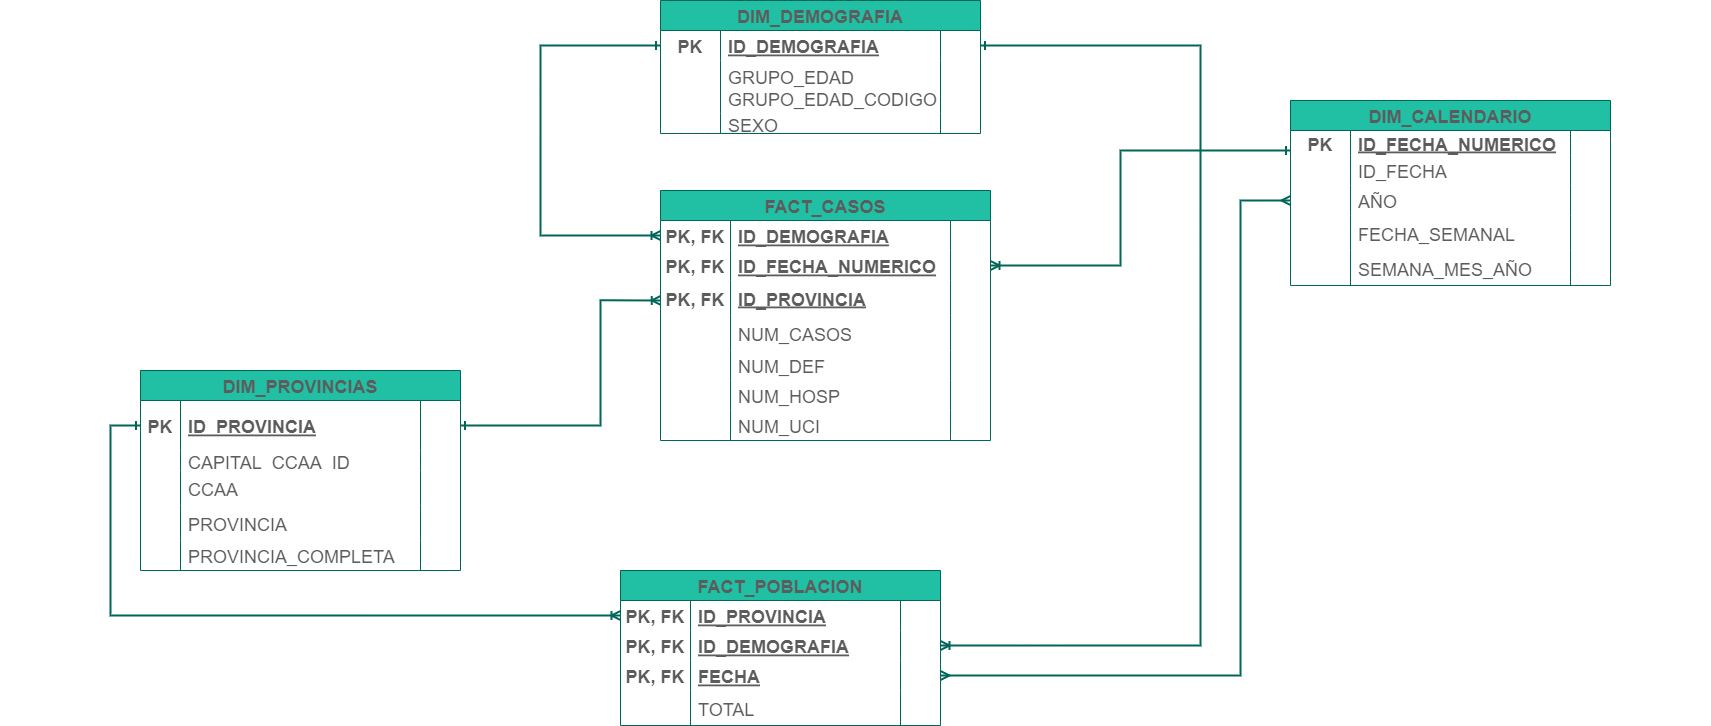
\includegraphics[scale=0.25]{img/casos_logico.png}
    \caption{Modelo lógico de casos.}
\end{figure}
\newpage

\subsubsection{Modelo físico de casos}
El modelo físico de casos es el siguiente:

\begin{figure}[h]
    \advance\leftskip-0.5cm \rightskip5cm
    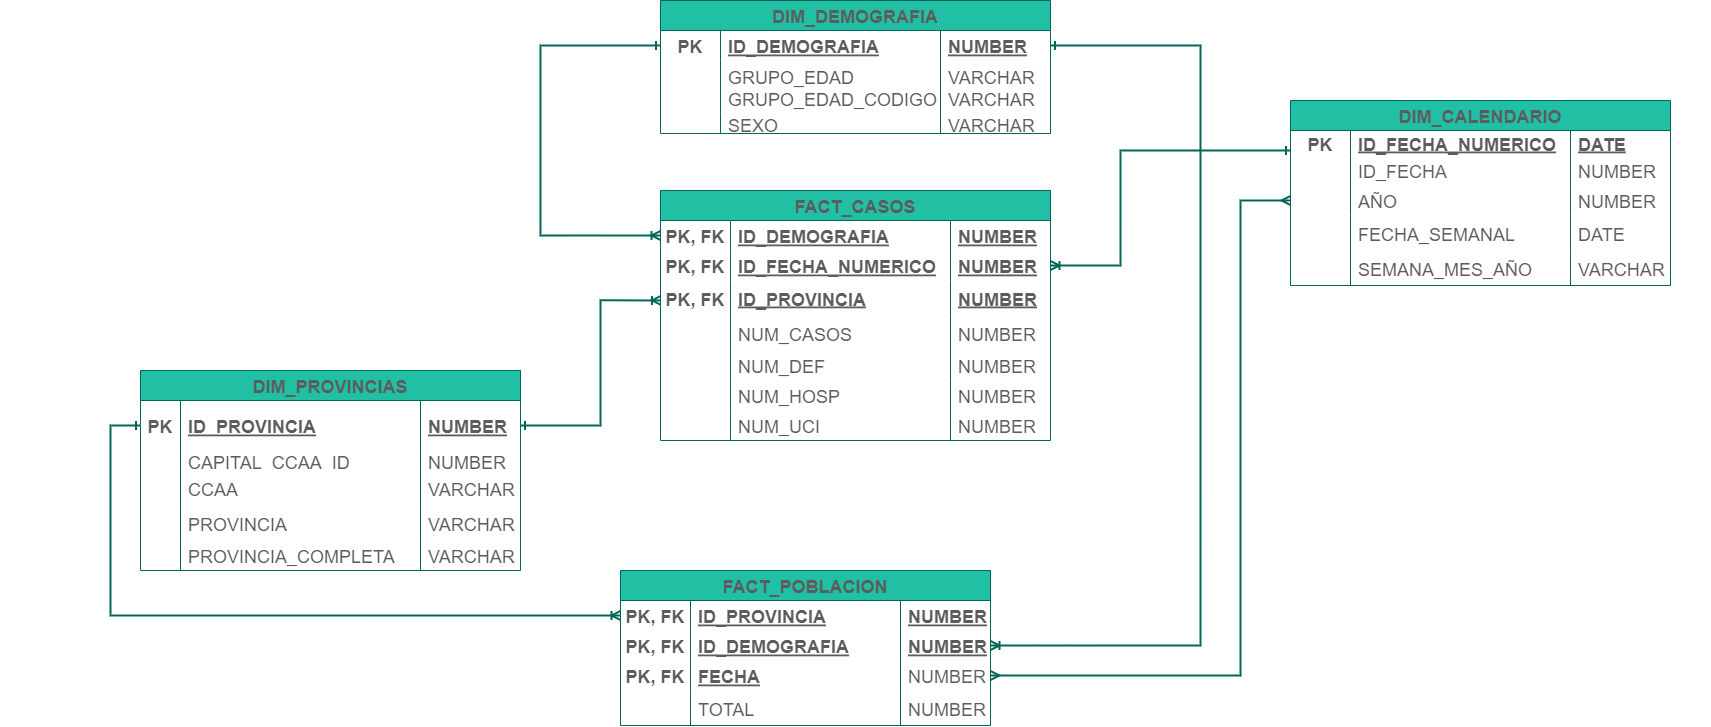
\includegraphics[scale=0.25]{img/casos_fisico.png}
    \caption{Modelo físico de casos.}
\end{figure}

\subsection{Hospitales}
Se ha realizado un modelado dimensional en tres fases: modelo conceptual, modelo lógico y modelo físico.

Los modelos de hospitales se utilizan en distintas hojas del cuadro de mandos, como en ingresos y altas hospitalarias, y camas hospitalarias.

\subsubsection{Modelo conceptual de hospitales}
El modelo conceptual de hospitales es el siguiente:

\imagen{hospitales_conc}{Modelo conceptual de hospitales.}

\subsubsection{Modelo lógico de hospitales}
El modelo lógico de hospitales es el siguiente:

\begin{figure}[h]
    \advance\leftskip-2cm \rightskip5cm
    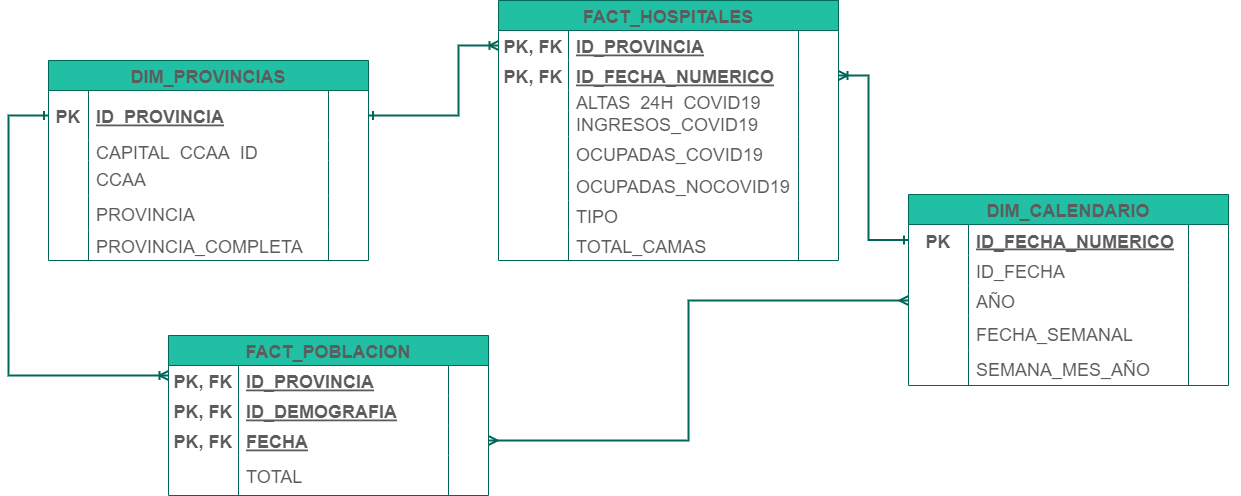
\includegraphics[scale=0.65]{img/hospitales_logico.png}
    \caption{Modelo lógico de hospitales.}
\end{figure}
\newpage

\subsubsection{Modelo físico de hospitales}
El modelo físico de hospitales es el siguiente:
\begin{figure}[h]
    \advance\leftskip-1cm \rightskip5cm
    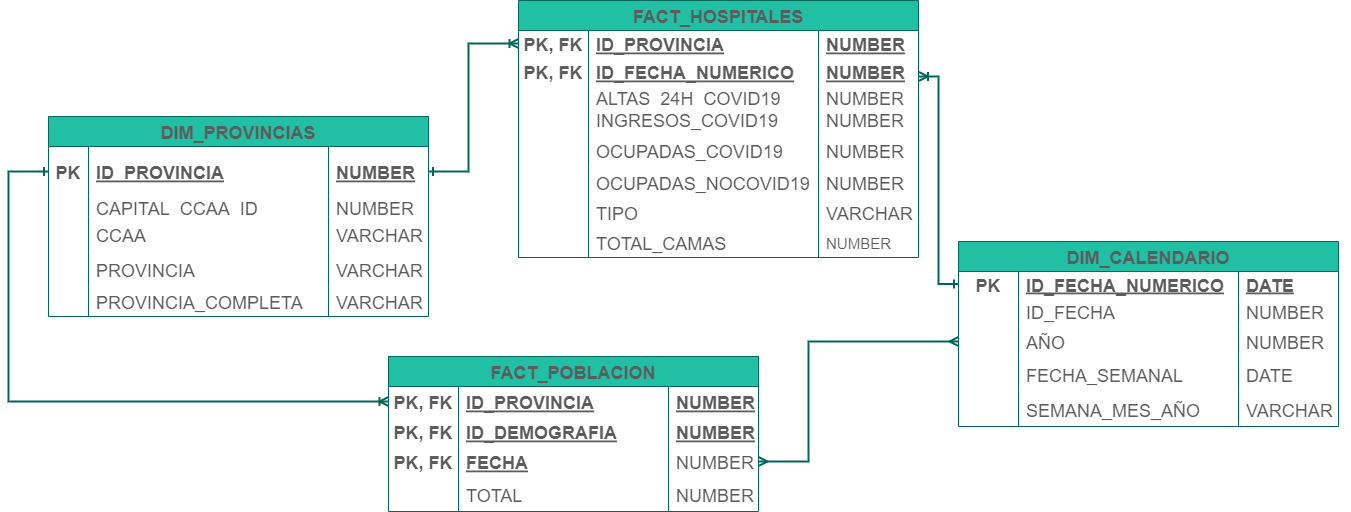
\includegraphics[scale=0.6]{img/hospitales_fisico.png}
    \caption{Modelo físico de hospitales.}
\end{figure}

\subsection{Residencias}
Se ha realizado un modelado dimensional en tres fases: modelo conceptual, modelo lógico y modelo físico.

Los modelos de residencias se utilizan la hoja del cuadro de mandos de residencias.

\subsubsection{Modelo conceptual de residencias} El modelo conceptual de residencias es el siguiente:
\imagen{residencias_conc}{Modelo conceptual de residencias.}

\subsubsection{Modelo lógico de residencias}
El modelo lógico de residencias es el siguiente:

\begin{figure}[h]
    \advance\leftskip-1.5cm \rightskip5cm
    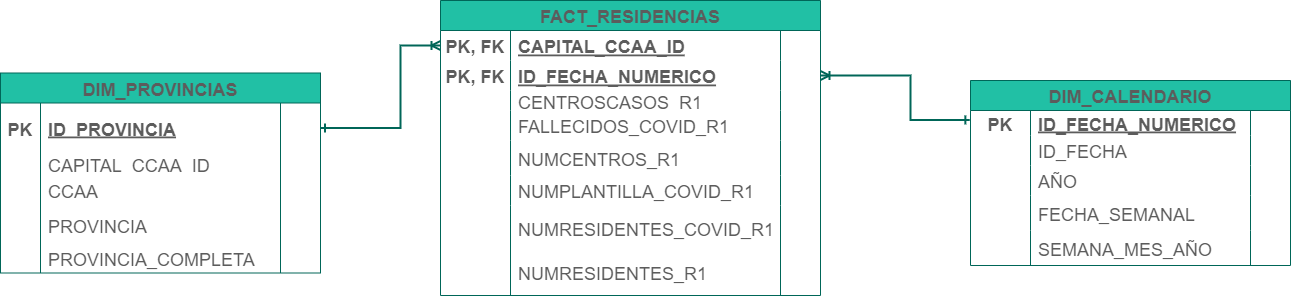
\includegraphics[scale=0.6]{img/residencias_logico.png}
    \caption{Modelo lógico de residencias.}
\end{figure}

\subsubsection{Modelo físico de residencias}
El modelo físico de residencias es el siguiente:

\begin{figure}[h]
    \advance\leftskip-0.5cm \rightskip5cm
    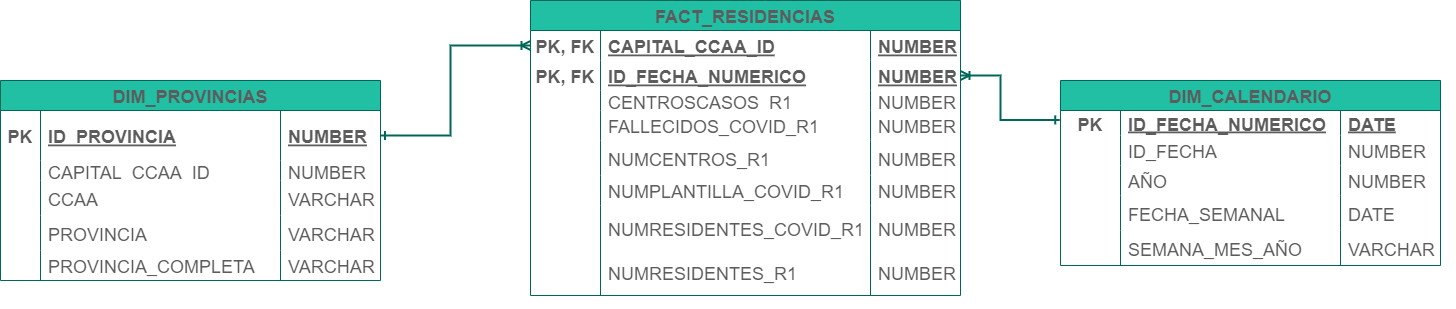
\includegraphics[scale=0.5]{img/residencias_fisico.png}
    \caption{Modelo físico de residencias.}
\end{figure}
\newpage

\subsection{Modelo final}
De esta forma el modelo final obtenido se compone de:

\begin{itemize}
    \item Casos: en esta tabla se almacena el número de casos, el número de defunciones, el número de hospitalizaciones y el número de casos en la UCI. Estos datos vienen agrupados en las siguientes columnas: identificador de demografía, identificador de fecha, identificador de provincia. Es una tabla de hechos, por lo tanto, se usarán sus datos para realizar cálculos.
    \item Provincias: en esta tabla se almacenan todas las provincias de España, cada provincia tiene los siguientes campos: el identificador de cada provincia, el código ISO de la provincia, la comunidad autónoma a la que pertenece, el código de la comunidad autónoma que pertenece y la respectiva capital de esa comunidad autónoma. Esta tabla es una dimensión y, por tanto, se usará para filtrar los cálculos que se hagan con las tablas de hecho.
    \item Demografía: en esta tabla se almacenan los datos demográficos, específicamente, el sexo y el grupo de edad, por tanto, esta tabla contará con los siguientes campos: el identificador de demografía, el grupo de edad y sexo. Esta tabla es una dimensión y por tanto se usará para filtrar los cálculos que se hagan con las tablas de hecho.
    \item Calendario: en esta tabla se almacenan las fechas de los datos contenidos en alguna de las tablas de hecho. Los campos de esta tabla son: el identificador de fecha y año, la fecha, el día de la semana, el día, el mes, el mes y año, el mes y año de forma numérica, la semana, la semana y mes, el trimestre, el trimestre y año, y el mes de forma numérica. Esta tabla es una dimensión y, por tanto, se usará para filtrar los cálculos que se hagan con las tablas de hecho.
    \item Población: en esta tabla se almacenan los datos sobre la población y está agrupada mediante las siguientes columnas: el identificador de demografía, el identificador del año, el identificador de la provincia. Es una tabla de hechos, por lo tanto, se usarán sus datos para realizar cálculos.
    \item Hospitales: en esta tabla se almacenan los datos sobre la situación en los hospitales: el número de altas en Covid-19 en las últimas 24 horas, el número de ingresos por Covid-19, el número de camas ocupadas por Covid-19, el tipo de hospitalización, el número total de camas en el hospital correspondiente, agrupados por el identificado de fecha y el identificador de provincia. Es una tabla de hechos, por lo tanto, se usarán sus datos para realizar cálculos.
    \item Residencias: en esta tabla se almacenan los datos sobre la situación en las residencias:  el número de centros, el número de plantilla Covid-19, el número de residentes con Covid-19, y el número de residentes, agrupadas por el identificador de fecha y el identificador de la capital de la comunidad autónoma.
\end{itemize}

\begin{figure}[h]
    \advance\leftskip-2cm \rightskip5cm
    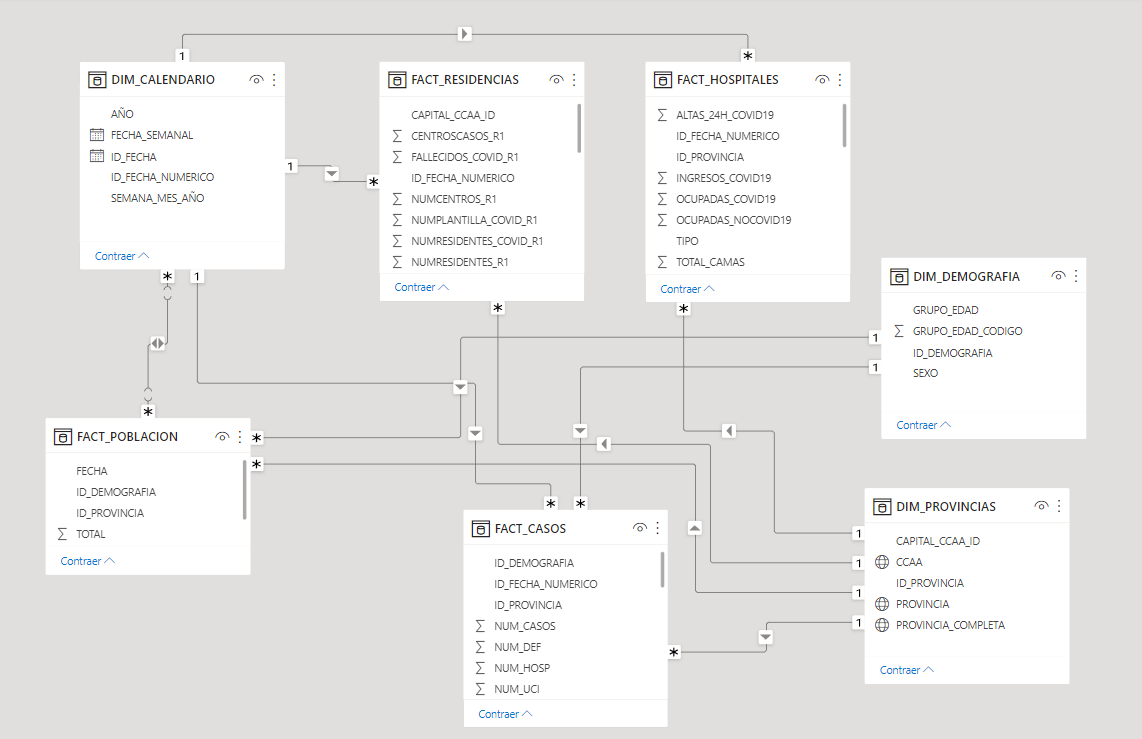
\includegraphics[scale=0.7]{img/modelo-final.PNG}
    \caption{Modelo final.}
\end{figure}
\section{Diseño procedimental}
En esta parte del anexo se muestra la ejecución de la arquitectura mediante diagramas de secuencia principalmente.

\subsection{Extracción}
Este primer diagrama de secuencia representa el proceso de extracción de los datos, desde su fuente hasta el data lake, donde se realizará la carga de los datos.
\imagen{extracción}{Diagrama de secuencia de extracción de datos.}

\subsection{Carga}
Este diagrama de secuencia representa el proceso de carga de los datos desde el data lake hasta la data warehouse Snowflake, concretamente su base de datos RAW.
\imagen{carga}{Diagrama de secuencia de carga de datos.}

\subsection{Transformación}
Este diagrama de secuencia representa el proceso de transformación dbt, en el que se recogen los datos crudos desde Snowflake, desde la base de datos RAW, realiza las transformaciones y los carga de nuevo en Snowflake, en la base de datos ANALYTICS.
\imagen{transformación}{Diagrama de secuencia de transformación de datos.}
\subsubsection{DAG transformaciones dbt}
A continuación, se muestra el Grafo Dirigido Acíclico (DAG) mediante el cual hace dbt las transformaciones de sus modelos.

\begin{landscape}
\begin{figure}[h]
    \advance\leftskip-1.5cm \rightskip5cm
    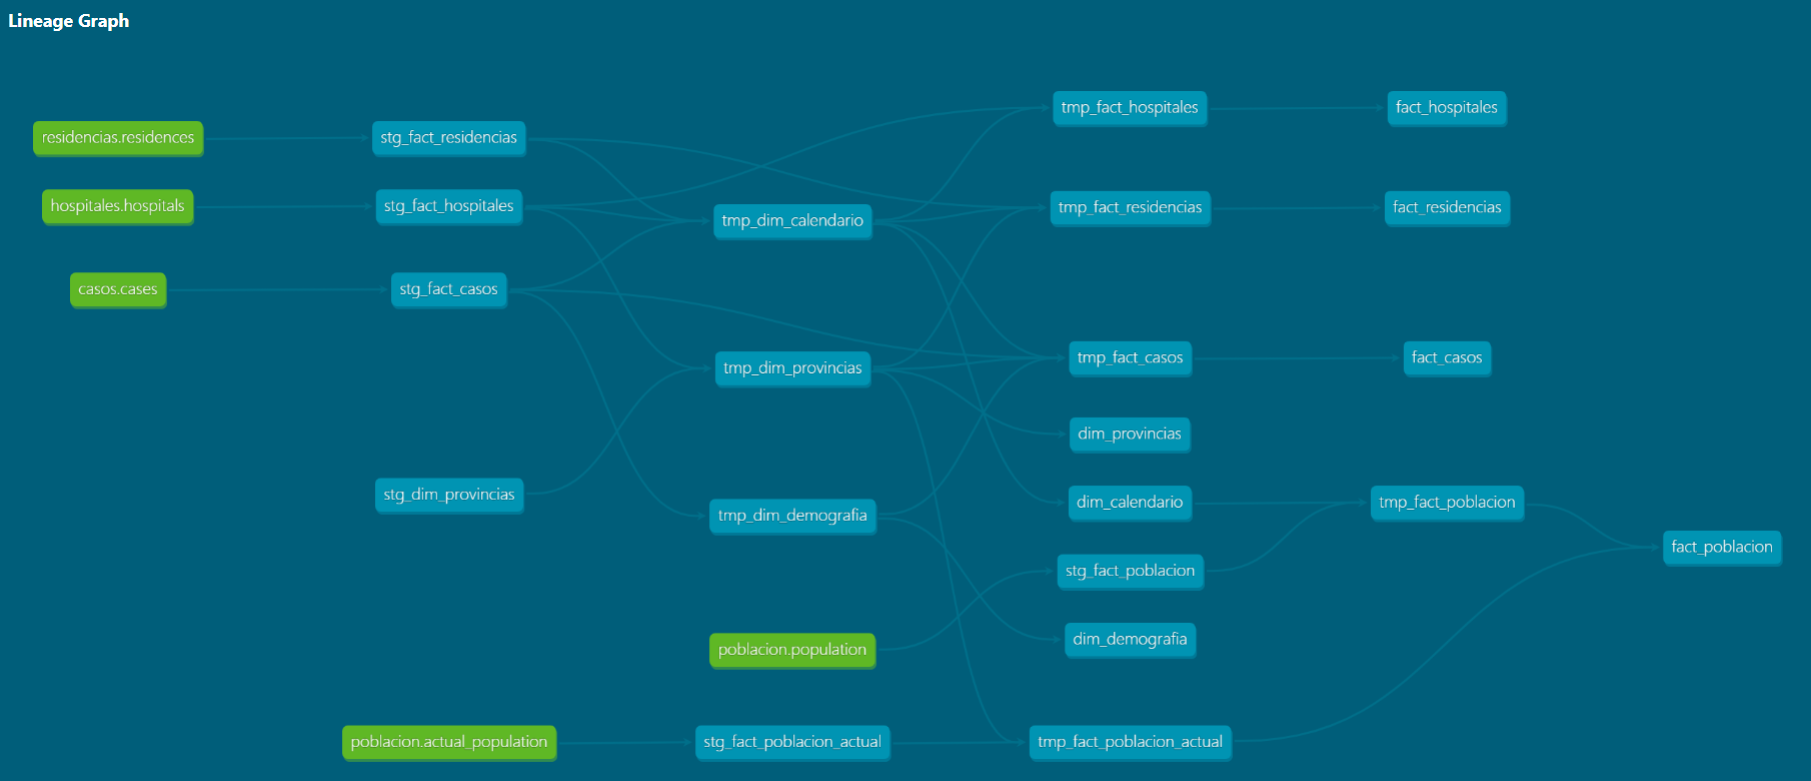
\includegraphics[scale=0.6]{img/DAG.PNG}
    \caption{Grafo Dirigido Acíclico (DAG) de las transformaciones.}
\end{figure}
\end{landscape}  

\subsection{Conexión de PowerBI a Datawarehouse}
Este diagrama de secuencia representa el proceso de conexión de PowerBI a snowflake, concretamente su base de datos ANALYTICS, mediante la cual se mantienen actualizados los datos en su cuadro de mandos.

\imagen{conexión}{Diagrama de secuencia de conexión de PowerBI a Datawarehouse.}

\subsection{Visualización de los datos por el usuario}
Este diagrama de secuencia representa el proceso de visualización de los datos por el usuario, y los pasos que este sigue.

\imagen{visualización}{Diagrama de secuencia de visualización de datos.}

\section{Diseño arquitectónico}

En este apartado se explicará el tipo de arquitectura que se ha escogido y que se ha seguido para tener un buen diseño.

\subsection{\emph{Modern Data Stack}}
Los Modern Data Stack \cite{Modern_Data_Stack} toman ventaja de los data warehouses en la nube, ya que traen mejoras en seguridad y elasticidad, y principalmente en el almacenamiento y procesamiento de grandes volúmenes de datos a gran velocidad y un coste muy bajo.

Los data warehouses solían ser un gran cuello de botella. Se usaban principalmente bases de datos relacionales basadas en filas como sus data warehouses, lo que no se adaptaba bien a las cargas de trabajo de análisis de datos, ya que distribuye los datos relacionados en varios discos o servidores. Incluso con tecnologías como Hadoop tardaban horas en ejecutarse y eran muy complicados de escribir y mantener. 

Además, debido al limitado poder de procesado de las antiguas data warehouses los ingenieros de datos solían hacer el trabajo de transformación antes de cargar los datos, lo que dio lugar al término ETL (\emph{Extract-Transform-Load}).

Ahora, con el avance de los data warehouse en la nube, gracias a su alto rendimiento, los ingenieros de datos pueden ejecutar consultas a escala de petabytes en minutos. 

Con un \emph{Modern Data Stack}, se pueden cargar los datos en el data warehouse en minutos y la transformación de datos se puede manejar de manera mucho más efectiva allí que en alguna capa de procesamiento externa (ELT, \emph{Extract-Load-Transform}).

Los princiapes beneficios de un Modern Data Stack por lo tanto son:

\begin{itemize}
	\item Modularidad: debido a que los Modern Data Stack consisten en varias tecnologías con puntos de conexión general, se pueden cambiar partes del stack a medida que las necesidades cambian, lo que ayuda a evitar el vendor lock-in.
	\item Velocidad: debido a los límites de procesamiento de las antiguas data warehouses, los pipelines podían llegar a tardar horas en ejecutarse, pero ahora con el Modern Data Stack y sus recursos de cómputo elásticos, ese trabajo puede hacerse en minutos.
	\item Coste: los costes de la tecnología en la nube son normalmente significativamente más baratos que su contraparte on-premise. Un data warehouse antiguo tendría que pagar por un servidor todo el tiempo, aparte de ser costoso y disponer de dificultades en su escalabilidad, al contrario que con un data warehouse en la nube, donde solo pagas por lo que usas y puedes escalar para cargas de trabajo masivas cuando sea necesario.
\end{itemize}

\subsection{ELT}
Los procesos ELT (\emph{Extract, load and transform}) \cite{ELT} consisten en la extracción, carga y transformación de datos. 

De manera que se diferencian de los procesos ETL en que los datos no se transforman al obtener los datos, sino que se guardan antes de ser procesados, es decir son almacenados en su formato inicial.

Esta nueva perspectiva está compuesta por:

\subsubsection{Modern ingestion}
La ingestión de datos \cite{Modern} comprende las fases de extracción de datos desde la fuente y la carga de estos mismo en el destino, la E y L del proceso ETL.

\subsubsection{Modern Storage}
El almacenamiento de datos \cite{Modern} se realiza mediante almacenes de datos en la nube, entre los que se incluyen \emph{Snowflake}.

Actualmente, estos almacenes de datos modernos presentan una serie de mejoras respecto a los anteriores, ya que permiten la ausencia de configuraciones de \emph{hardware}, y se caracterizan por su disponibilidad, rapidez y menor coste.

\subsubsection{Modern transformation}
La transformación moderna de datos \cite{Modern} convierte, limpia y agrega, entre otras funciones, los datos. Y todas estas acciones se realizan directamente sobre el data warehouse analítico.


\subsection{Aplicación en el proyecto}

Para el proyecto se ha construido la siguiente arquitectura:

\subsubsection{Ingestión de datos}

La primera parte de la arquitectura del Modern Data Stack es la ingestión, correspondiente al EL, la extracción y carga de datos, del ELT. Para ello se han utilizado varias herramientas, ya que tenemos varias fuentes de datos que hay actualizar frecuentemente como los datos de los casos, los datos hospitalarios, etc. Hemos montado una estructura capaz de extraer y cargar los datos diaria y automáticamente, de forma que siempre tengamos lo datos actualizados. Estas herramientas son las siguientes:

\begin{itemize}
	\item Google cloud: \cite{google_cloud} es un espacio virtual por el que se puede realizar una serie de tareas que antes requerían de hardware o software, y que ahora usan la nube de Google como única forma de acceso, almacenamiento y gestión de datos. Especificamente se han utilizado los siguientes servicios:
	\begin{itemize}
    	\item Cloud functions: \cite{cloud_functions} es un servicio que sirve para crear aplicaciones sin servidores dentro de Google Cloud, dando respuesta a la demanda de eventos que puedan ocurrir en cualquier sitio. Lo positivo de este servicio es que abonarás solo por lo que uses, ósea el tiempo que tu código se esté ejecutando, por lo tanto, es buena opción para proyectos pequeños. En este caso lo hemos utilizado para realizar un script de Phyton \cite{Python} que extrae desde URLs de fuentes oficiales del estado, .csv con los datos que queremos actualizar diariamente de la pandemia para llevarlos a Amazon S3, nuestro data lake, dónde reunimos los datos antes de cargarlos en nuestro data warehouse.
    	\item Cloud Scheduler: \cite{cloud_scheduler} es un programador de trabajos cron administrado. Permite programar prácticamente cualquier trabajo, desde trabajos por lotes y de macrodatos, hasta operaciones de infraestructura de nube y mucho más. Es el servicio que usamos para que se ejecuten nuestros scripts de phyton de forma diaria.
    	\item Pub|Sub: \cite{pub/sub} este servicio permite que otros servicios se comuniquen de forma asíncrona. Se usa para las canalizaciones de integración de datos y estadísticas de transmisión a fin de transferir y distribuir datos. Es igual de efectivo que un middleware orientado a la mensajería para la integración de servicio, o como una cola a fin de paralelizar tareas. Lo usamos para que se pueda comunicar Cloud Scheduler con el script de python programado en Cloud functions.
    \end{itemize}
	\item Amazon S3: \cite{Amazon} es un servicio que ofrece el almacenamiento de elementos a partir de una interfaz de servicio web. Se puede almacenar cualquier tipo de objeto, por lo que se le puede dar varios usos. En nuestro caso será usado como un data lake. El script de python comentado en el apartado anterior, va a cargar en este data lake los .csv que queremos cargar en el data warehouse. 
	\item Fivetran: \cite{Fivetran} es una herramienta que permite a las compañías extraer datos de varias fuentes y cargarlas en un destino, normalmente un data warehouse en la nube. Estas tareas de integración están automatizadas y usan conectores de datos preconstruidos, que hay que configurar para que se conecten a las fuentes y el destino de los datos. En nuestro caso, lo usaremos para cargar nuestros datos del data lake creado en Amazon S3 en nuestra datewarehouse en Snowflake. Esta tarea también está automatizada, realizándose de manera diaria, de forma que tendremos siempre los datos actualizados. 

\end{itemize}

\subsubsection{Almacenamiento de datos}

Para almacenar los datos se ha utilizado la datawarehouse en la nube snowflake \cite{Snowflake}, la cual utiliza un repositorio de datos centralizado para datos persistentes, accesible desde todos los nodos del data warehouse, y que cuando va a procesar las consultas cada clúster almacena una porción de los datos localmente para procesarlos en paralelo.

En nuestro caso vamos a tener dos bases de datos. Una llamada RAW, con el esquema COVID, donde se cargarán desde Amazon S3 los datos crudos. Y otra llamada ANALYTICS dónde estarán los datos transformados. Esta base de datos tendrá dos esquemas, DBT\_JOSEDANIELBALLESTER, donde se cargarán los datos desde entorno de desarrollo, y el esquema ANALYTICS, donde se cargarán los datos del entorno de producción, desde el cual se cargará posteriormente a PowerBI para su explotación.

La arquitectura de Snowflake tiene 3 capas:

\begin{itemize}
	\item Database storage: en esta capa están los datos, una vez están en la nube, Snowflake los reorganiza en su propio formato para mejorar el rendimiento.
	\item Query processing: esta capa realiza las consultas mediante almacenes virtuales, cada uno de ellos es un cluster de varios nodos que trabajan en paralelo.
	\item Cloud services: son varios servicios que coordinan las actividades de Snowflake.
\end{itemize}

\subsubsection{Transformación de datos}

Para la transformación utilizaremos dbt, el cual se conectará con Snowflake, cogerá los datos desde la base de datos RAW y una vez realizadas las transformaciones, cargará los datos en la base de datos ANALYTICS.

Dbt \cite{dbt} es una herramienta de línea de comandos que permite desarrollar colaborativamente código de analítica. Es la herramienta que se encarga de las trasformaciones, la T del ELT, siguiendo las mejores prácticas de la ingeniería del software como la modularidad, portabilidad, la integración y distribución continua, la documentación, el control de versiones, y el testeo de cada modelo, permitiendo construir data pipelines robustos.

Dbt depende de SQL para transformar los datos, no le queda más remedio ya que, al estar transformando los datos directamente en la data warehouse en la nube, está delegando todo el trabajo pesado en su motor. Aun así, dbt agrega funcionalidad de código como por ejemplo bucles, que no hay en SQL, gracias al template jinja, lo que permite escribir código más eficiente.

En su flujo de trabajo para las transformaciones se generan automáticamente grafos de dependencia y su ejecución se puede programar y automatizar en su entorno en la nube, cosa que se ha hecho, de forma que diariamente se van a realizar las transformaciones programadas sobre la base de datos RAW, cargándolas en la base de datos ANALYTICS, de forma que PowerBI tendrá siempre datos actualizados, de cómo mucho un día de antigüedad disponibles.

\subsubsection{Reporting}

Microsoft Power BI\cite{MPBI} es una herramienta que posibilita la conexión a distintas fuentes de datos locales o en la nube. De forma que se puede ajustar la información fácilmente, permitiendo producir tableros de control en tiempo real, e informes que incluyen la información óptima para la mejora del desarrollo de los resultados.
	
Así, Microsoft Power BI permite unir diferentes fuentes de datos, modelizar y analizar datos para después, presentarlos a través de paneles e informes; y que así puedan ser consultados de una manera fácil, atractiva e intuitiva.
	
Por ello, es una herramienta usada para la fase de análisis y creación de paneles e informes, que permite realizar diversos gráficos que ayudan a visualizar los datos y sacar insights de forma cómoda y flexible gracias a la posibilidad de aplicar filtros dinámicos.

Nuestro panel va a estar alojado en la nube, de forma que va a ser posible acceder a él a través de una URL, además al estar conectado directamente a Snowflake, hemos programado que de forma diaria se actualice automáticamente cargando los datos alojados en la base de datos ANALYTICS.

\begin{figure}[h]
    \advance\leftskip-2cm \rightskip5cm
    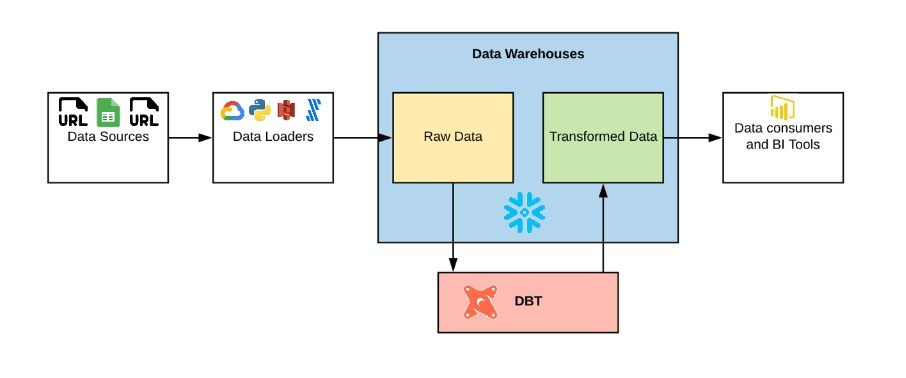
\includegraphics[scale=0.55]{img/dis_arq.jpeg}
    \caption{Diseño arquitectónico.}
\end{figure}

\section{Diseño de interfaces}
Para la realización del proyecto, primero se desarrolló un prototipo de las diferentes interfaces del cuadro de mandos con la herramienta de diseño Canva. De esta forma se asentaron las ideas de cómo iba a ser el diseño del cuadro de mandos en un principio.

\newpage
El primero que se diseñó fue el prototipo resumen de la situación general de Covid-19. 

\begin{figure}[h]
    \advance\leftskip-1cm \rightskip5cm
    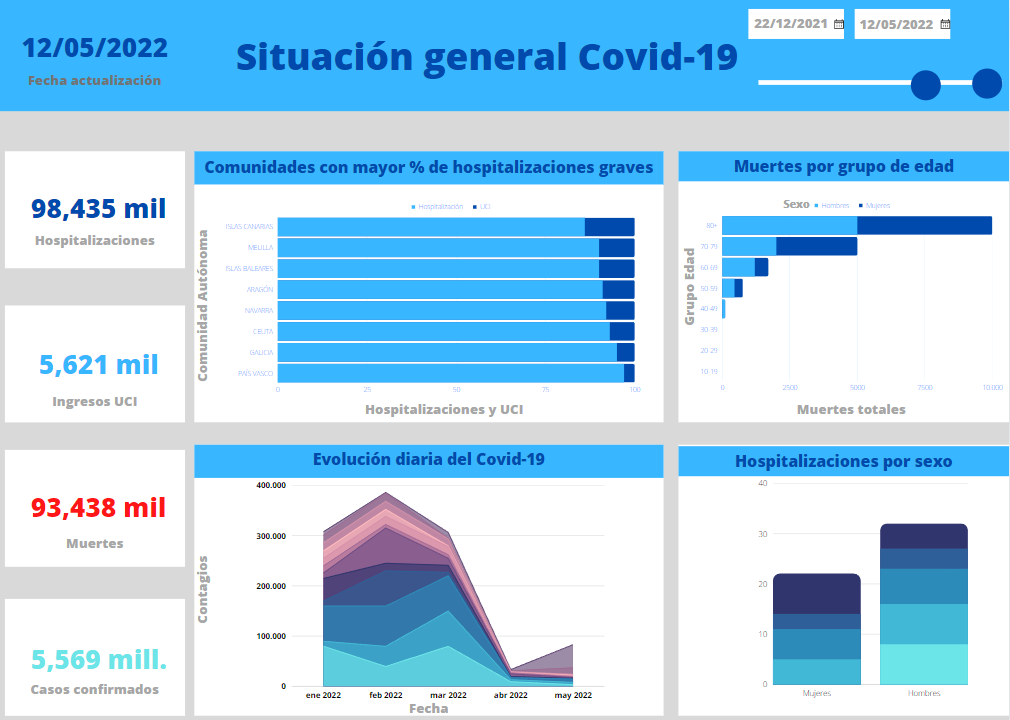
\includegraphics[scale=0.7]{img/prototipo_resumen.PNG}
    \caption{Prototipo resumen.}
\end{figure}

Éste constaría de cinco tarjetas con datos sobre la fecha de actualización, hospitalizaciones, ingresos UCI, muertes, y casos confirmados. 

También, constaría de cuatro gráficos principales que facilitarían la visualización de información sobre las comunidades con mayor porcentaje de hospitalizaciones graves, las muertes por grupo de edad, la evolución diaria del Covid-19, y las hospitalizaciones por sexo, respectivamente.

Además, permitiría el filtrado de la información mediante un filtro de fecha.

\newpage
A continuación, se incluye la interfaz final del resumen de la situación general del Covid-19.

\begin{figure}[h]
    \advance\leftskip-0.5cm \rightskip5cm
    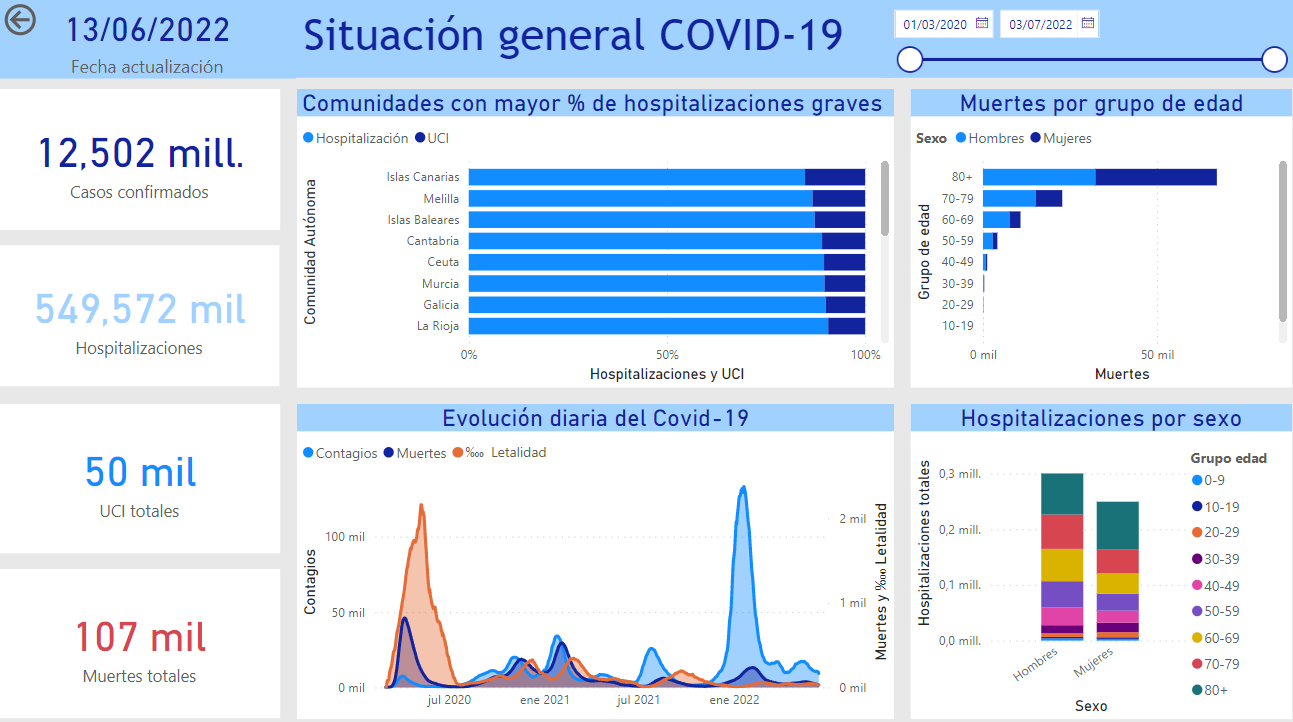
\includegraphics[scale=0.55]{img/powerBI_resumen.PNG}
    \caption{Diseño resumen.}
\end{figure}

Se puede ver como la interfaz final es prácticamente igual al prototipo inicial, por lo que se ha conseguido el correcto seguimiento del prototipo.

\newpage
Después, se diseñó el prototipo de la incidencia acumulada. 

\begin{figure}[h]
    \advance\leftskip-1cm \rightskip5cm
    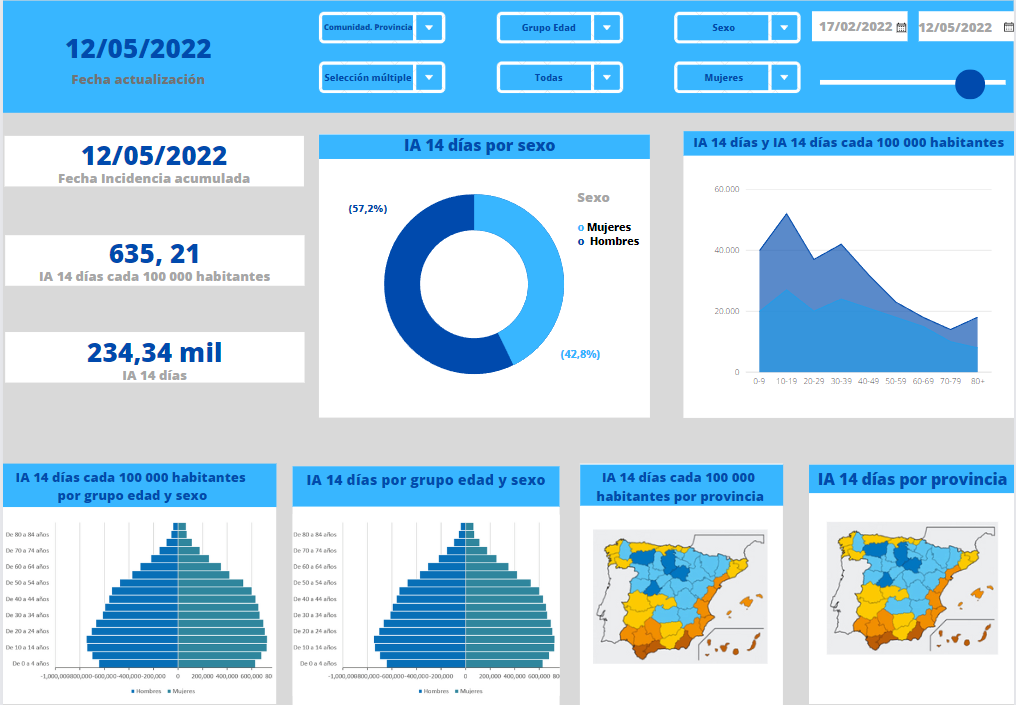
\includegraphics[scale=0.7]{img/prototipo_IA.png}
    \caption{Prototipo incidencia acumulada.}
\end{figure}

Éste constaría de cuatro tarjetas con datos sobre la fecha de actualización, la fecha de incidencia acumulada, la incidencia acumulada a 14 días cada 100.000 habitantes y la incidencia acumulada a 14 días. 

También constaría de cuatro gráficos y dos mapas  coropléticos, que facilitarían la visualización de información sobre la incidencia acumulada a 14 días por sexo, la incidencia acumulada a 14 días cada 100.000 habitantes, la incidencia acumulada a 14 días cada 100.000 habitantes por grupo de edad y sexo, la incidencia acumulada a 14 días por grupo de edad y sexo, la incidencia acumulada a 14 días cada 100.000 habitantes por provincia, y la incidencia acumulada a 14 días por provincia, respectivamente.

Además, permitiría el filtrado de la información mediante filtros de fecha, comunidades, provincia, grupo de edad y sexo.

\newpage
A continuación, se incluye la interfaz final de la incidencia acumulada. 

\begin{figure}[h]
    \advance\leftskip-0.5cm \rightskip5cm
    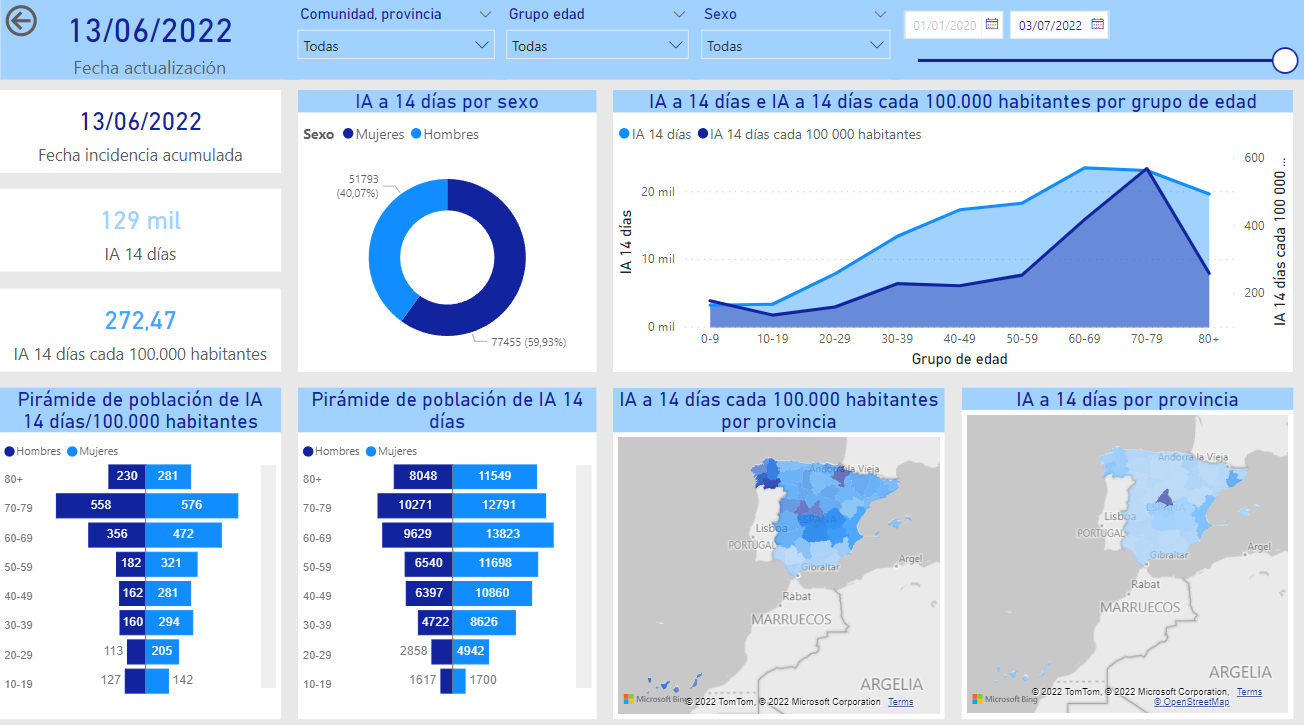
\includegraphics[scale=0.55]{img/powerBI_IA.PNG}
    \caption{Diseño incidencia acumulada.}
\end{figure}

A pesar de que la interfaz final es muy similar al prototipo inicial, difieren en una serie de aspectos como algún título de gráfico.

\newpage
Luego, se diseñó el prototipo de casos y muertes. 

\begin{figure}[h]
    \advance\leftskip-1cm \rightskip5cm
    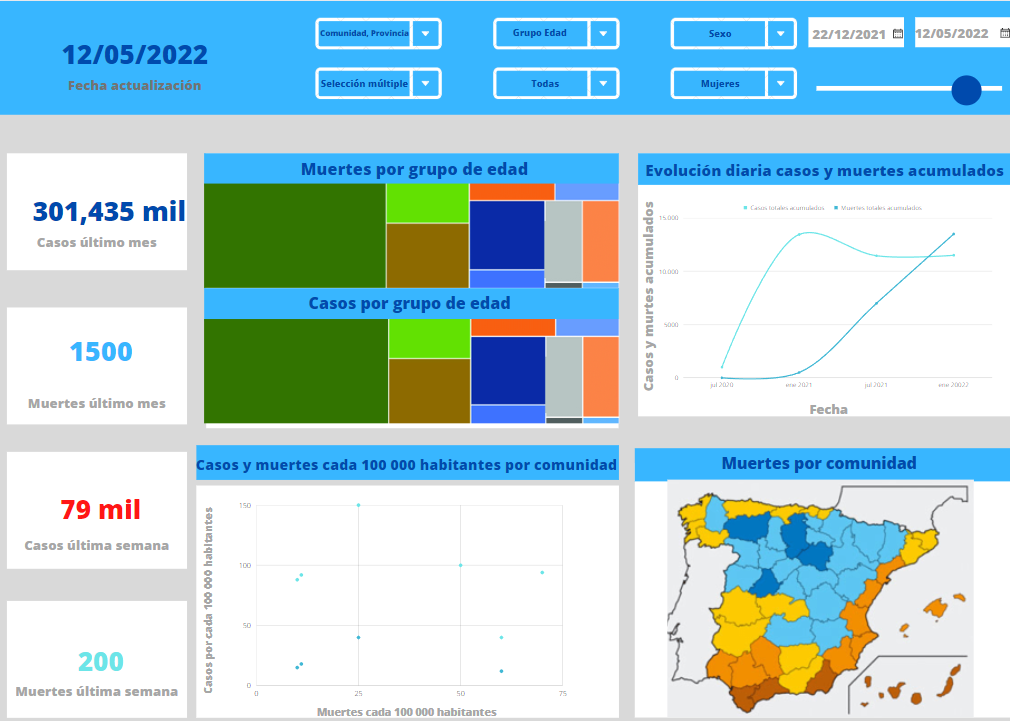
\includegraphics[scale=0.7]{img/prototipo_casosYmuertes.PNG}
    \caption{Prototipo casos y muertes.}
\end{figure}

Éste constaría de cinco tarjetas con datos sobre la fecha de actualización, los casos del último mes, las muertes del último mes, los casos de la última semana, y las muertes de la última semana. 

También constaría de tres gráficos y un mapa coroplético, que facilitarían la visualización de información sobre las muertes por grupo de edad, los casos por grupo de edad, la evolución diaria de los casos y muertes acumuladas, los casos y muertes cada 100.000 habitantes por comunidad, y las muertes por comunidad, respectivamente.

Además, permitiría el filtrado de la información mediante filtros de fecha, comunidades, provincia, grupo de edad y sexo.

\newpage 
A continuación, se incluye la interfaz final de los casos y muertes. 

\begin{figure}[h]
    \advance\leftskip-0.5cm \rightskip5cm
    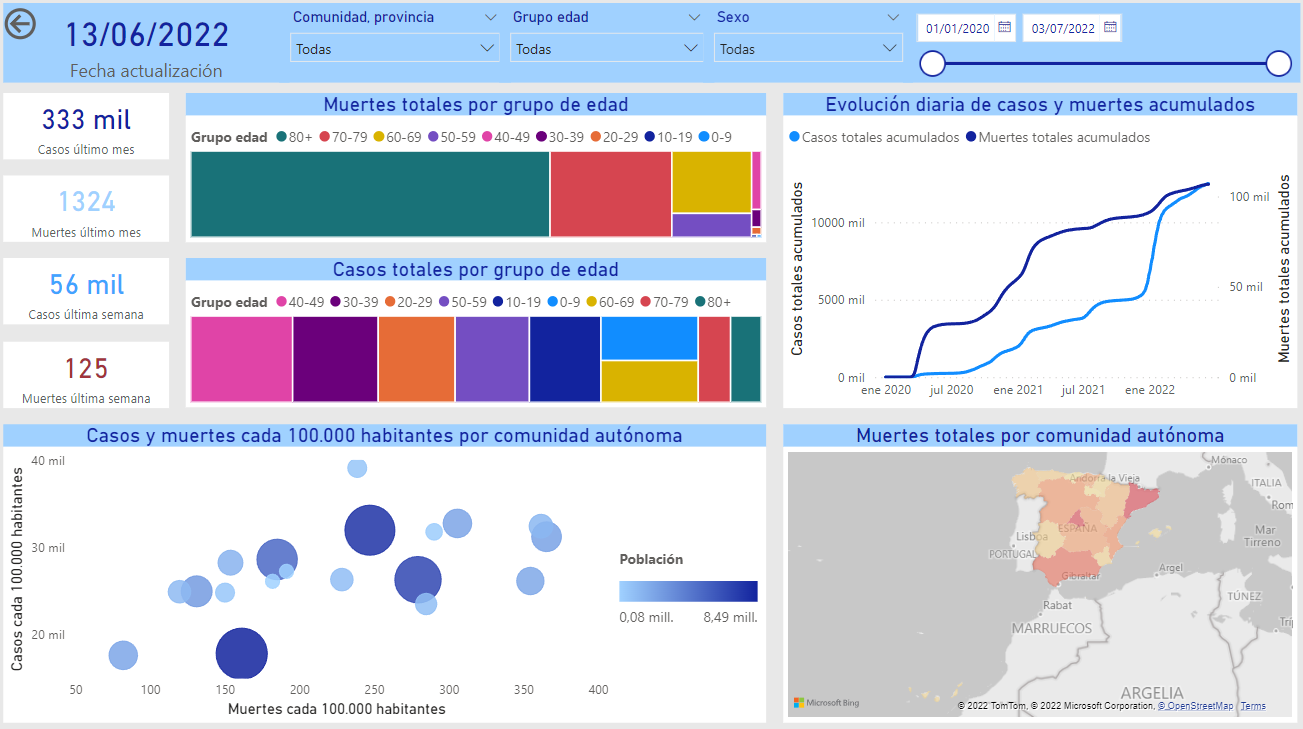
\includegraphics[scale=0.55]{img/powerBI_casosYmuertes.PNG}
    \caption{Diseño casos y muertes.}
\end{figure}

A pesar de que la interfaz final es muy similar al prototipo inicial, difieren en una serie de aspectos como algún título de gráfico.

\newpage
Posteriormente, se diseñó el prototipo de ingresos y altas hospitalarias. 

\begin{figure}[h]
    \advance\leftskip-1cm \rightskip5cm
    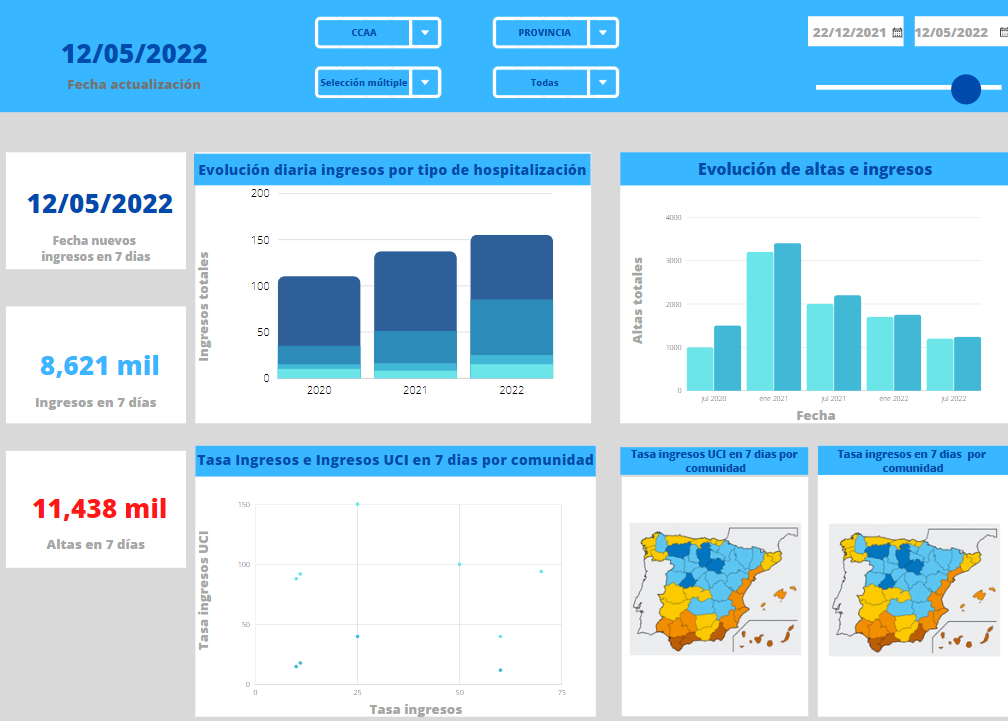
\includegraphics[scale=0.7]{img/prototipo_ingresosYaltas.PNG}
    \caption{Prototipo ingresos y altas hospitalarias.}
\end{figure}

Éste constaría de cuatro tarjetas con datos sobre fecha de actualización, la fecha de nuevos ingresos en 7 días, los ingresos en 7 días, y las altas en 7 días. 

También constaría de tres gráficos y dos mapas coropléticos, que facilitarían la visualización de información sobre la evolución diaria de ingresos por tipo de hospitalizaciones, la evolución de altas e ingresos, la tasa de ingresos y la tasa de ingresos UCI en 7 días por comunidad, la tasa de ingresos UCI en 7 días por comunidad, y la tasa de ingresos en 7 días por comunidad, respectivamente. 

Además, permitiría el filtrado de la información mediante filtros de fecha, comunidades autónomas y de provincia.

\newpage
A continuación, se incluye la interfaz final de los ingresos y altas hospitalarias. 

\begin{figure}[h]
    \advance\leftskip-0.5cm \rightskip5cm
    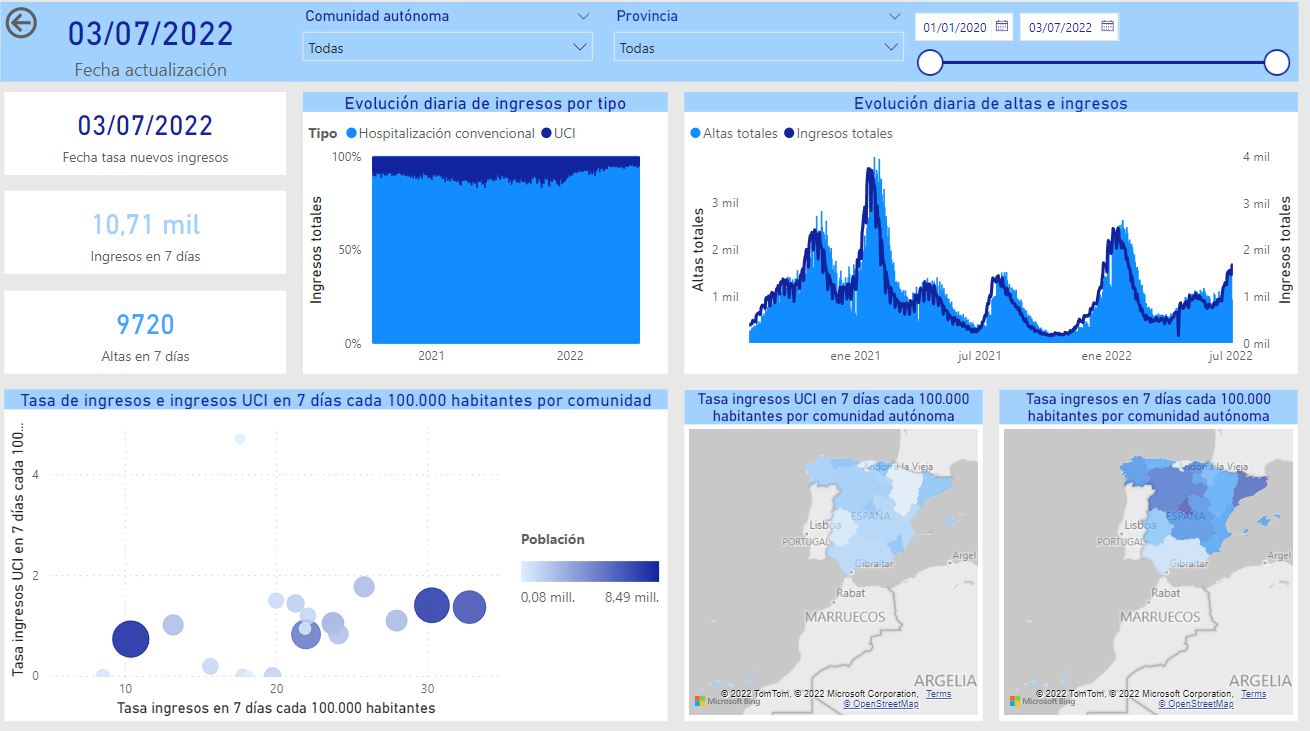
\includegraphics[scale=0.55]{img/powerBI_ingresosYaltas.PNG}
    \caption{Diseño ingresos y altas hospitalarias.}
\end{figure}

A pesar de que la interfaz final es muy similar al prototipo inicial, difieren en una serie de aspectos como en algunos títulos y tipos de gráficos.

\newpage
Seguidamente, se diseñó el prototipo de camas hospitalarias. 

\begin{figure}[h]
    \advance\leftskip-1cm \rightskip5cm
    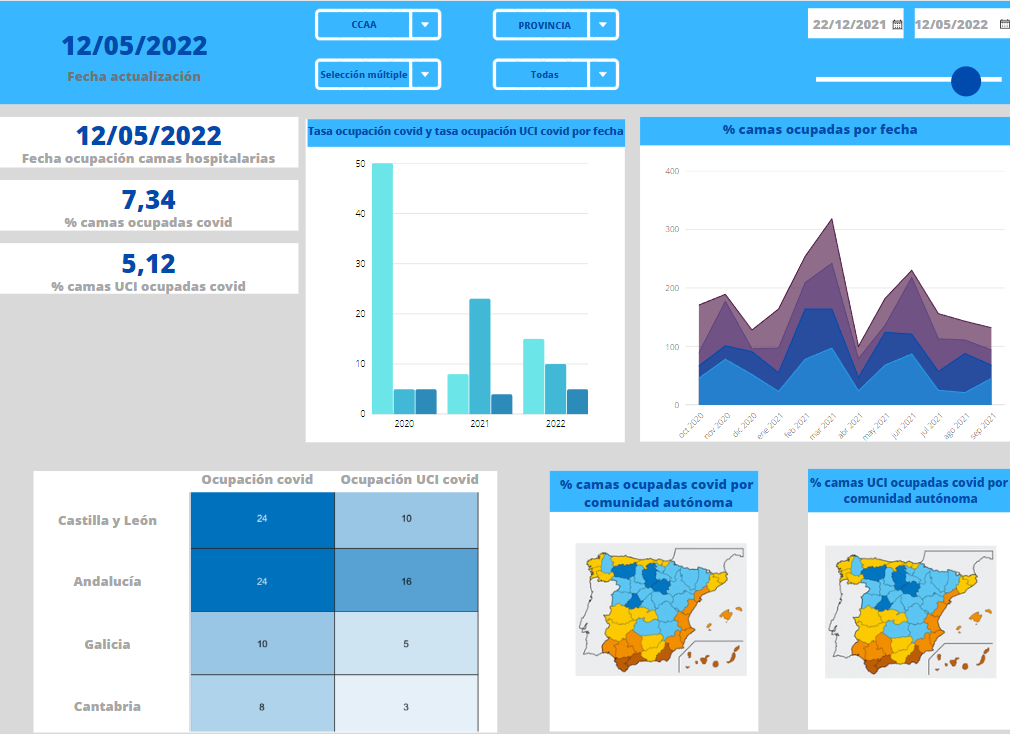
\includegraphics[scale=0.7]{img/prototipo_camas.PNG}
    \caption{Prototipo camas hospitalarias.}
\end{figure}

Éste constaría de cuatro tarjetas con datos sobre fecha de actualización, la fecha de ocupación de camas hospitalarias, el porcentaje de camas ocupadas por Covid-19, y el porcentaje de camas UCI ocupadas por Covid-19. 

También constaría de dos gráficos, una matriz y dos mapas coropléticos, que facilitarían la visualización de información sobre la tasa de ocupación covid y tasa de ocupación UCI por fecha, el porcentaje de camas ocupadas por fecha, la ocupación por Covid-19 y la ocupación UCI por Covid-19 por comunidades autónomas, el porcentaje de camas ocupadas por Covid-19 por comunidad autónoma, y el porcentaje de camas UCI ocupadas por Covid-19 por comunidad autónoma, respectivamente. 

Además, permitiría el filtrado de la información mediante filtros de fecha, comunidades autónomas y de provincia.

\newpage
A continuación, se incluye la interfaz final de las camas hospitalarias.

\begin{figure}[h]
    \advance\leftskip-0.5cm \rightskip5cm
    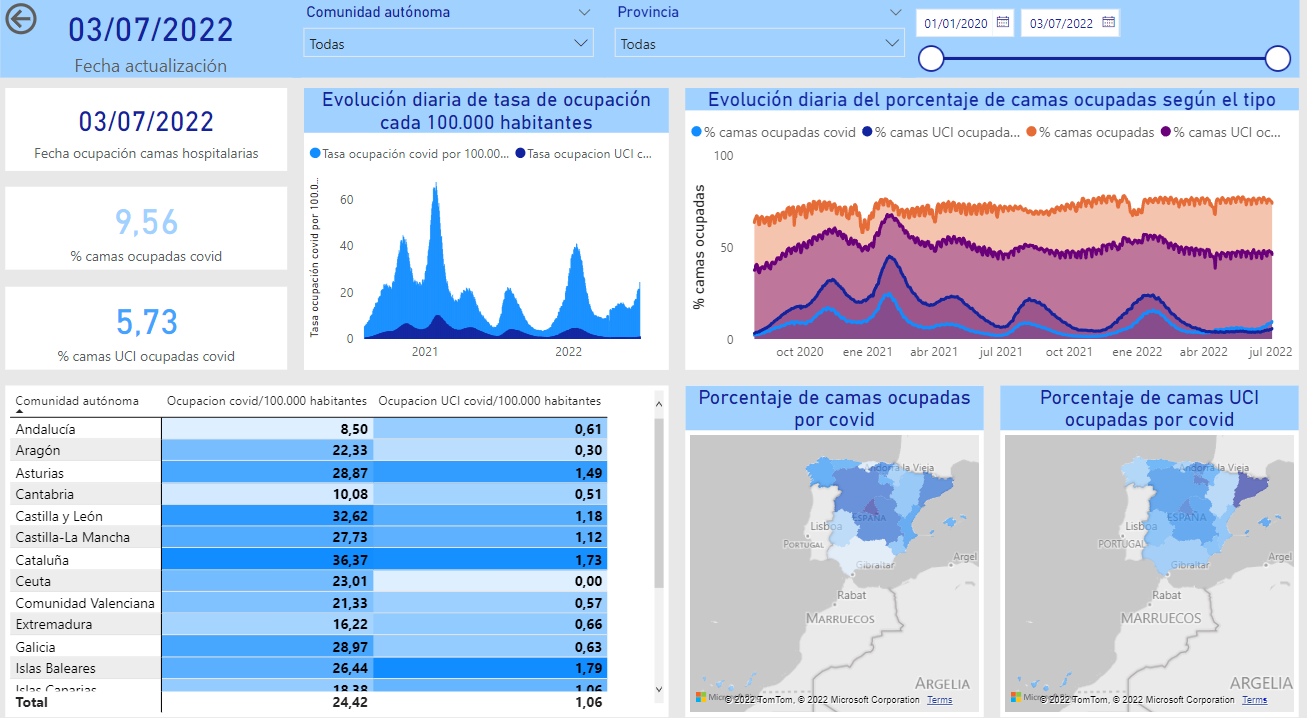
\includegraphics[scale=0.55]{img/powerBI_camas.PNG}
    \caption{Diseño camas hospitalarias.}
\end{figure}

A pesar de que la interfaz final es muy similar al prototipo inicial, difieren en una serie de aspectos como en algunos títulos y tipos de gráficos.

\newpage
Por último, se diseñó el prototipo de residencias. 

\begin{figure}[h]
    \advance\leftskip-1cm \rightskip5cm
    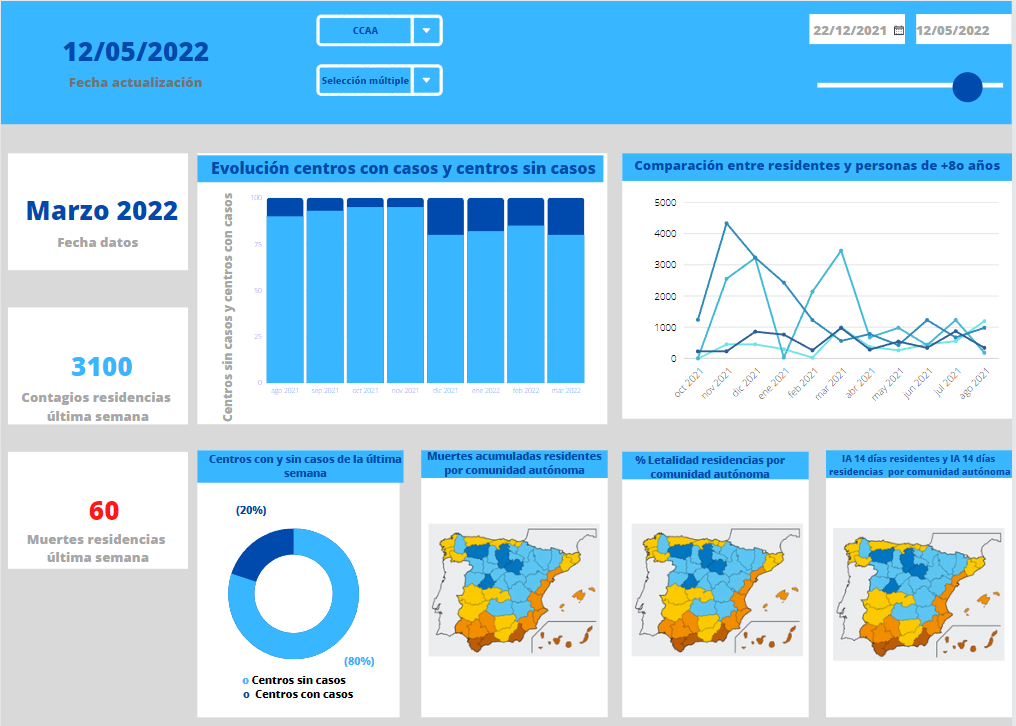
\includegraphics[scale=0.7]{img/prototipo_residencias.PNG}
    \caption{Prototipo residencias}
\end{figure}

Éste constaría de cuatro tarjetas con datos sobre la fecha de actualización, la fecha de los datos, los contagios en las residencias en la última semana, y las muertes en las residencias en la última semana. 

También constaría de tres gráficos y tres mapas coropléticos, que facilitarían la visualización de información sobre la evolución de los centros con casos y los centros sin casos, la comparación entre los residentes y personas de más de 80 años, los centros con casos y sin casos de la última semana, las muertes acumuladas de residentes  por comunidad autónoma, el porcentaje de letalidad de residentes por comunidad autónoma, y la incidencia acumulada a 14 días de los residentes por comunidad autónoma, respectivamente. 

Además, permitiría el filtrado de la información mediante un filtro de fecha y comunidades autónomas.

A continuación, se incluye la interfaz final de los ingresos y altas hospitalarias. 

\begin{figure}[h]
    \advance\leftskip-0.5cm \rightskip5cm
    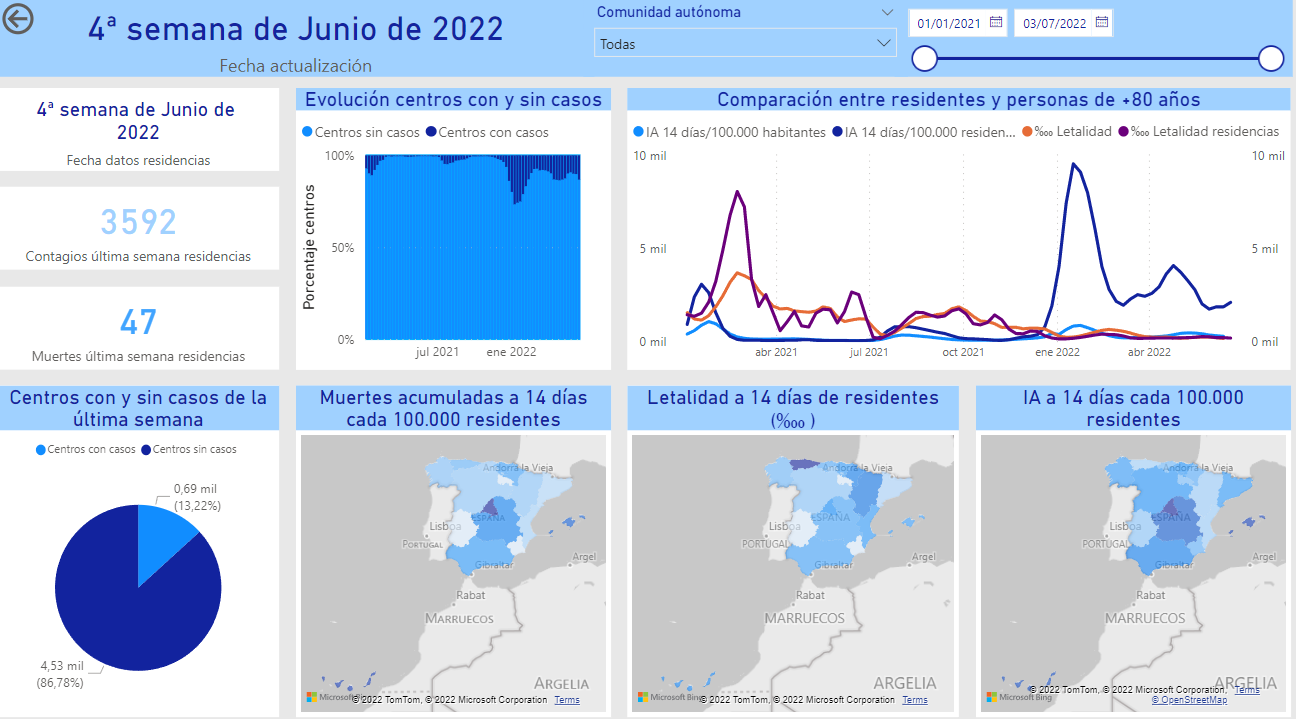
\includegraphics[scale=0.55]{img/powerBI_residencias.PNG}
    \caption{Diseño residencias}
\end{figure}

A pesar de que la interfaz final es muy similar al prototipo inicial, difieren en una serie de aspectos como algún título de gráfico.